

%\documentclass[a4paper]{jarticle}

\section{mpie.rb 円グラフの描画\label{sect:mpie}}
\index{mpie@mpie}

円グラフを描画するコマンドである。
x軸・y軸に展開する属性項目を指定することで、
1次元もしくは2次元の円グラフ行列を描画することができる。
グラフは単独のHTMLファイルとして出力されるので、
一般的なブラウザで表示が可能である。

入力データには、表\ref{tbl:mpie_input2}のようなCSVを用いる。
円グラフを構成する扇となる項目を構成要素項目といい、
\verb|f=|パラメータで指定する。
x軸・y軸に展開する属性項目は\verb|k=|パラメータで指定する。
\verb|k=|パラメータで1項目を指定すると1次元の(x軸に展開された)円グラフ行列が、
2項目を指定すると2次元の(x軸・y軸に展開された)円グラフ行列が描画される。
\verb|k=|パラメータを省略した場合は、1個の円グラフが描画される。

なお円グラフの描画には、内部的に
JavaScriptライブラリD3.js(Data-Driven Documents)を使用している。
D3.jsの詳細は公式ページ(\url{http://d3js.org/})を参照のこと。

また本コマンドを利用するためには、nysol/mcmdライブラリが必要となる。

\begin{table}[http]
\begin{center}
\caption{都道府県と年代別の個体数\label{tbl:mpie_input2}}
{\small
\begin{tabular}[t]{ccr}
\hline
Pref&Age&Population \\
\hline
奈良&10&310504\\
奈良&20&552339\\
奈良&30&259034\\
奈良&40&450818\\
奈良&50&1231572\\
奈良&60&1215966\\
奈良&70&641667\\
北海道&10&310504\\
北海道&20&252339\\
北海道&30&859034\\
北海道&40&150818\\
北海道&50&9231572\\
北海道&60&4215966\\
北海道&70&341667\\
\hline
\end{tabular}
}
\end{center}
\end{table}

\newpage
\subsection{書式}
\begin{verbatim}
  mpie.rb [i=] f= v= [o=] [k=] [title=] [pr=] [cc=] [--help]
\end{verbatim}

\begin{table}[htbp]
{\small
\begin{tabular}{ll}
\verb|i=|        & 入力データファイル名(CSV形式)\\
\verb|f=|        & 構成要素項目名を指定する。\\
                 & データにnullが含まれる場合は無視する。\\
\verb|v=|        & 構成比項目(円グラフの円弧の長さを決定する項目)を指定する。\\
                 & データにnullが含まれる場合は0として扱う。\\
                 & 先頭の0は無視する。数字以外の場合はエラーとなる。\\
\verb|o=|        & 出力ファイル名(HTMLファイル)\\
\verb|k=|        & x軸・y軸に展開する属性項目名を2つ以内で指定する。\\
                 & 省略した場合は円グラフを1つ作成する。\\
                 & 項目を1つ指定した場合は1次元の円グラフ行列を、\\
                 & 項目を2つ指定した場合は2次元の円グラフ行列を作成する。\\
\verb|title=|    & グラフのタイトル文字列を指定する。\\
\verb|pr=|       & 円グラフの半径を指定する(デフォルトは160)。\\
\verb|cc=|       & 1行に表示する円グラフの最大数を指定する(デフォルトは5)。\\
                 & 1次元の円グラフ行列のときのみ指定できる。\\
\verb|--help|    & ヘルプの表示\\
\end{tabular} 
}
\end{table} 

なお\verb|mpie.rb|コマンドには、
\verb|f=|パラメータや\verb|k=|パラメータで指定した項目を
自動的に並べ替える機能はない。
グラフに表示したい順に、あらかじめ並べ替えておく必要がある。

\subsection{利用例}
\subsubsection*{例1: 円グラフを1つ描画する}

\verb|dat1.csv|ファイルの\verb|Age|を構成要素項目に、
\verb|Population|を構成比項目として円グラフを1つ描画する。

\begin{Verbatim}[baselinestretch=0.6,frame=single]
$ more dat1.csv
Age,Population
10,310504
20,552339
30,259034.5555
40,0450818
50,1231572
60,1215966
70,641667
$ mpie.rb i=dat1.csv v=Population f=Age o=result1.html
#END# mpie.rb i=dat1.csv v=Population f=Age o=result1.html;
\end{Verbatim}

以下の円グラフが描画される。

ブラウザで表示した円グラフにマウスカーソルを置くと、
構成要素項目とその構成比がポップアップで表示される。
グラフはマウスによるドラッグ操作で移動することができ、
またマウスのスクロール操作によって拡大縮小もできる。

\begin{flushleft}
\fbox{
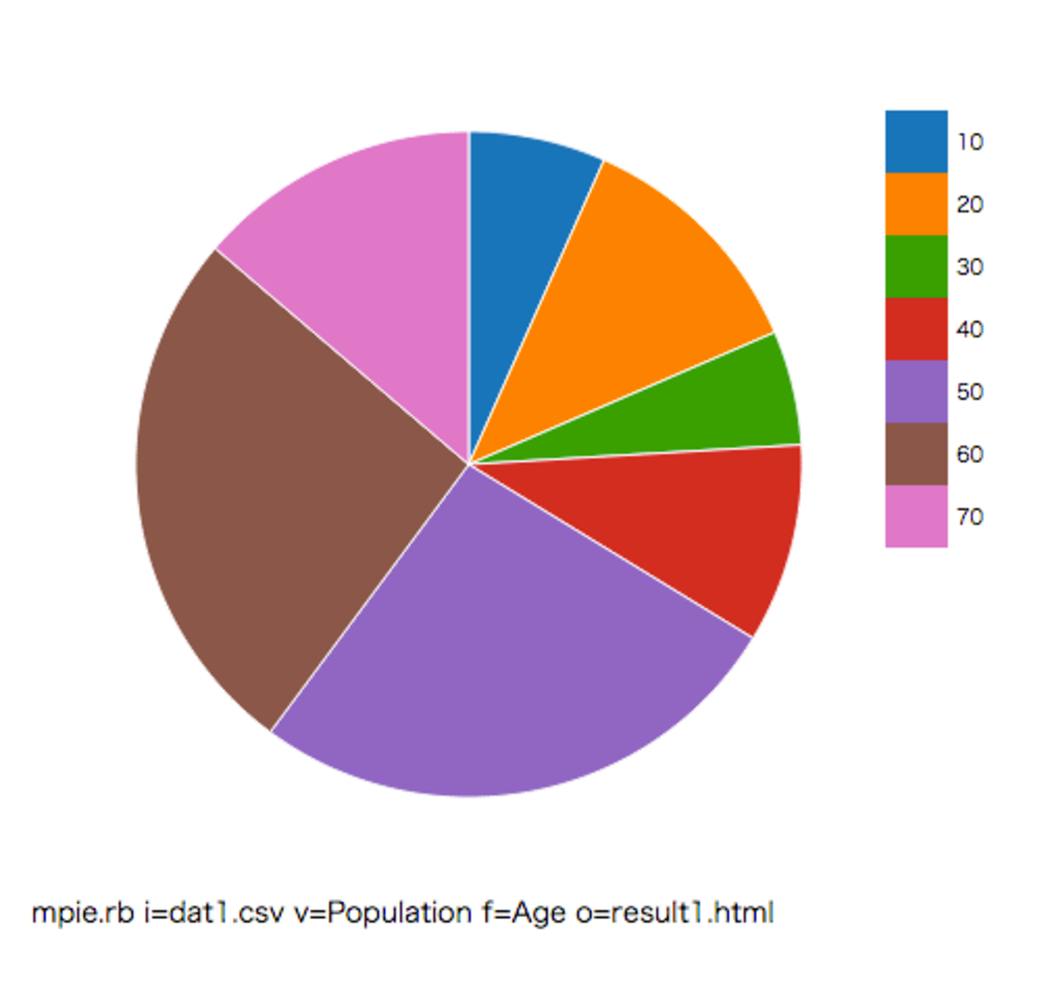
\includegraphics[scale=0.7]{figure/mpie1.eps}
}
\end{flushleft}

\subsubsection*{例2: 1次元の円グラフ行列を描画する}

\verb|dat2.csv|ファイルの\verb|Age|を構成要素項目に、
\verb|Population|を構成比項目として円グラフを描画する。
\verb|k=|パラメータに\verb|Pref|項目を指定しているので、
\verb|Pref|項目の値をx軸(横方向)に展開した1次元の円グラフ行列が描画される。
\verb|title=|パラメータでグラフのタイトルも指定している。

\begin{Verbatim}[baselinestretch=0.5,frame=single]
$ more dat2.csv
Pref,Age,Population
奈良,10,310504
奈良,20,552339
奈良,30,259034
奈良,40,450818
奈良,50,1231572
奈良,60,1215966
奈良,70,641667
北海道,10,310504
北海道,20,252339
北海道,30,859034
北海道,40,150818
北海道,50,9231572
北海道,60,4215966
北海道,70,341667
$ mpie.rb i=dat2.csv k=Pref v=Population f=Age o=result2.html
 title=奈良と北海道の年代ごとの人口
#END# mpie.rb i=dat2.csv k=Pref v=Population f=Age o=result2.html 
title=奈良と北海道の年代ごとの人口;
\end{Verbatim}

以下の円グラフ行列が描画される。

\begin{flushleft}
\fbox{
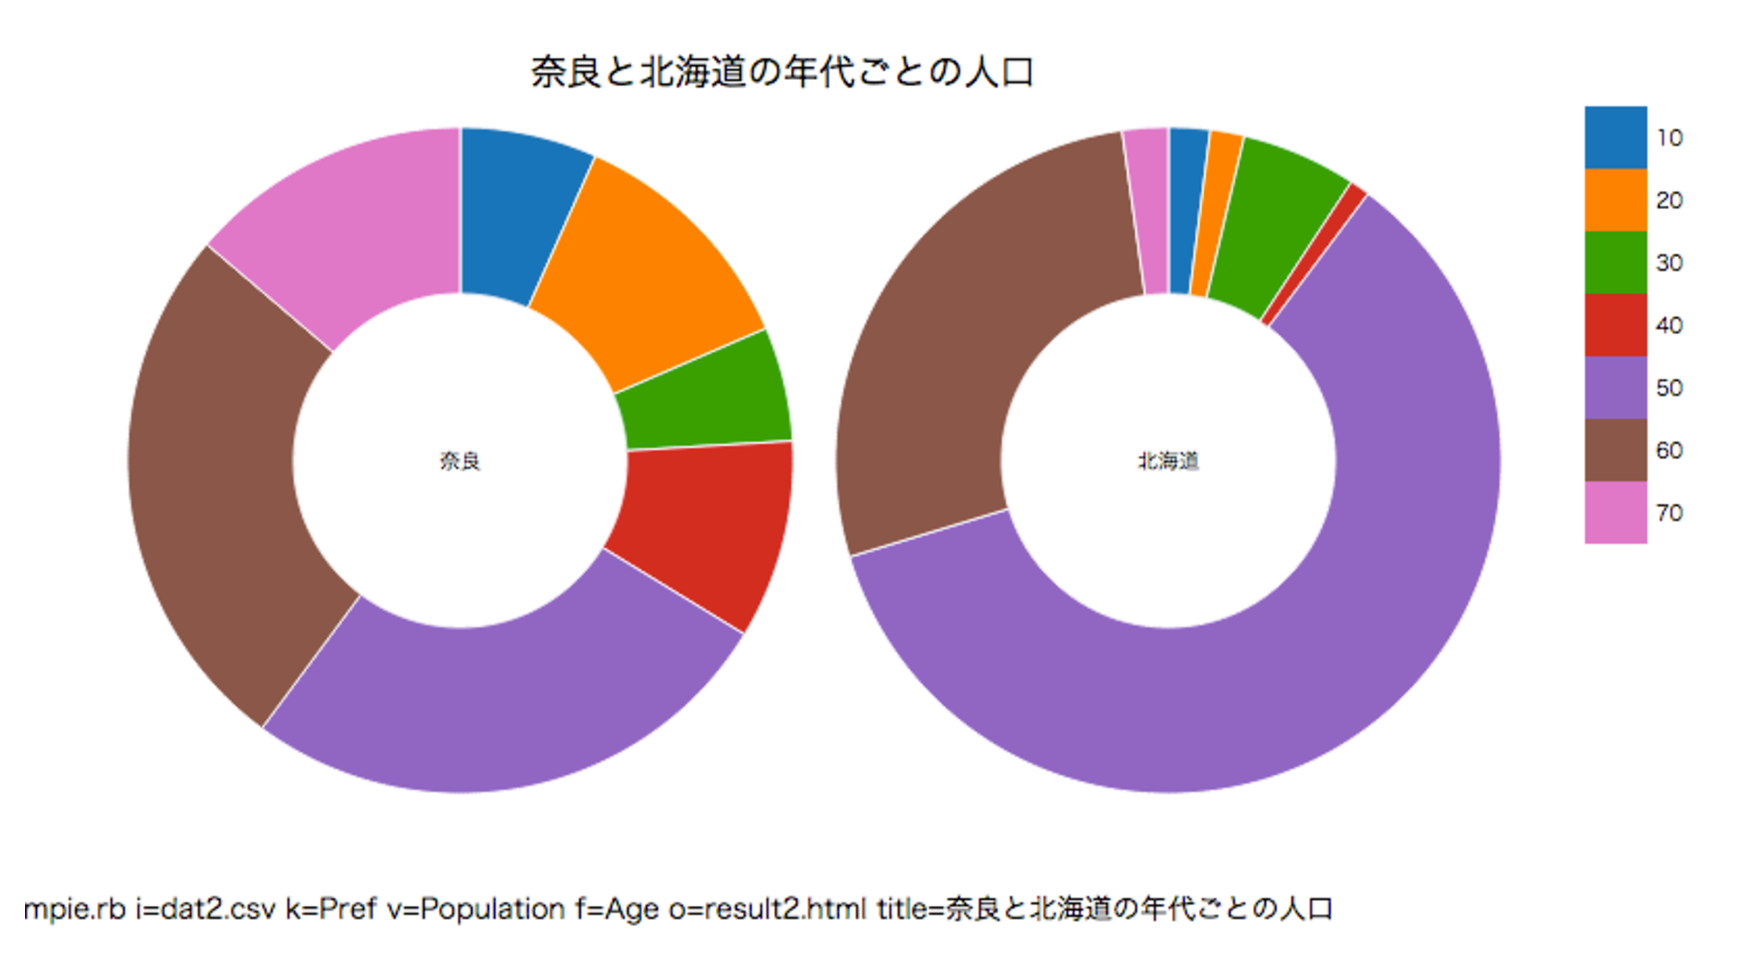
\includegraphics[scale=0.5]{figure/mpie2.eps}
}
\end{flushleft}

\subsubsection*{例3: 2次元の円グラフ行列を描画する}
\verb|dat3.csv|ファイルの\verb|テーマパーク名|を構成要素項目、
\verb|Number|を構成比項目とし、\verb|pr=|パラメータに半径100を指定して円グラフを描画する。
\verb|k=|パラメータに\verb|Gender|と\verb|Age|項目を指定しているので、
\verb|Gender|項目の値をx軸(横方向)に、
\verb|Age|項目の値をy軸(縦方向)に展開した2次元の円グラフ行列が描画される。

\begin{noautoxspacing}
\begin{Verbatim}[baselinestretch=0.5,frame=single]
$ more dat3.csv
Gender,Age,テーマパーク名,Number
男性,30,デズニ,100
男性,30,UFJ,59
男性,30,梅屋敷,180
男性,40,デズニ,200
男性,40,UFJ,3
男性,40,梅屋敷,10
男性,50,デズニ,110
男性,50,UFJ,40
女性,30,梅屋敷,100
女性,30,デズニ,80
女性,30,UFJ,200
女性,40,デズニ,90
女性,40,UFJ,80
女性,40,梅屋敷,120
女性,50,デズニ,99
女性,50,UFJ,80
女性,50,梅屋敷,110
$ mpie.rb i=dat3.csv k=Gender,Age v=Number f=テーマパーク名 o=result3.html
 title=性別と年代ごとのテーマパーク訪問回 pr=100
#END# mpie.rb i=dat3.csv k=Gender,Age v=Number f=テーマパーク名 o=result3.html 
title=性別と年代ごとのテーマパーク訪問回 pr=100;
\end{Verbatim}
\end{noautoxspacing}

以下の円グラフ行列が描画される。

\begin{flushleft}
\fbox{
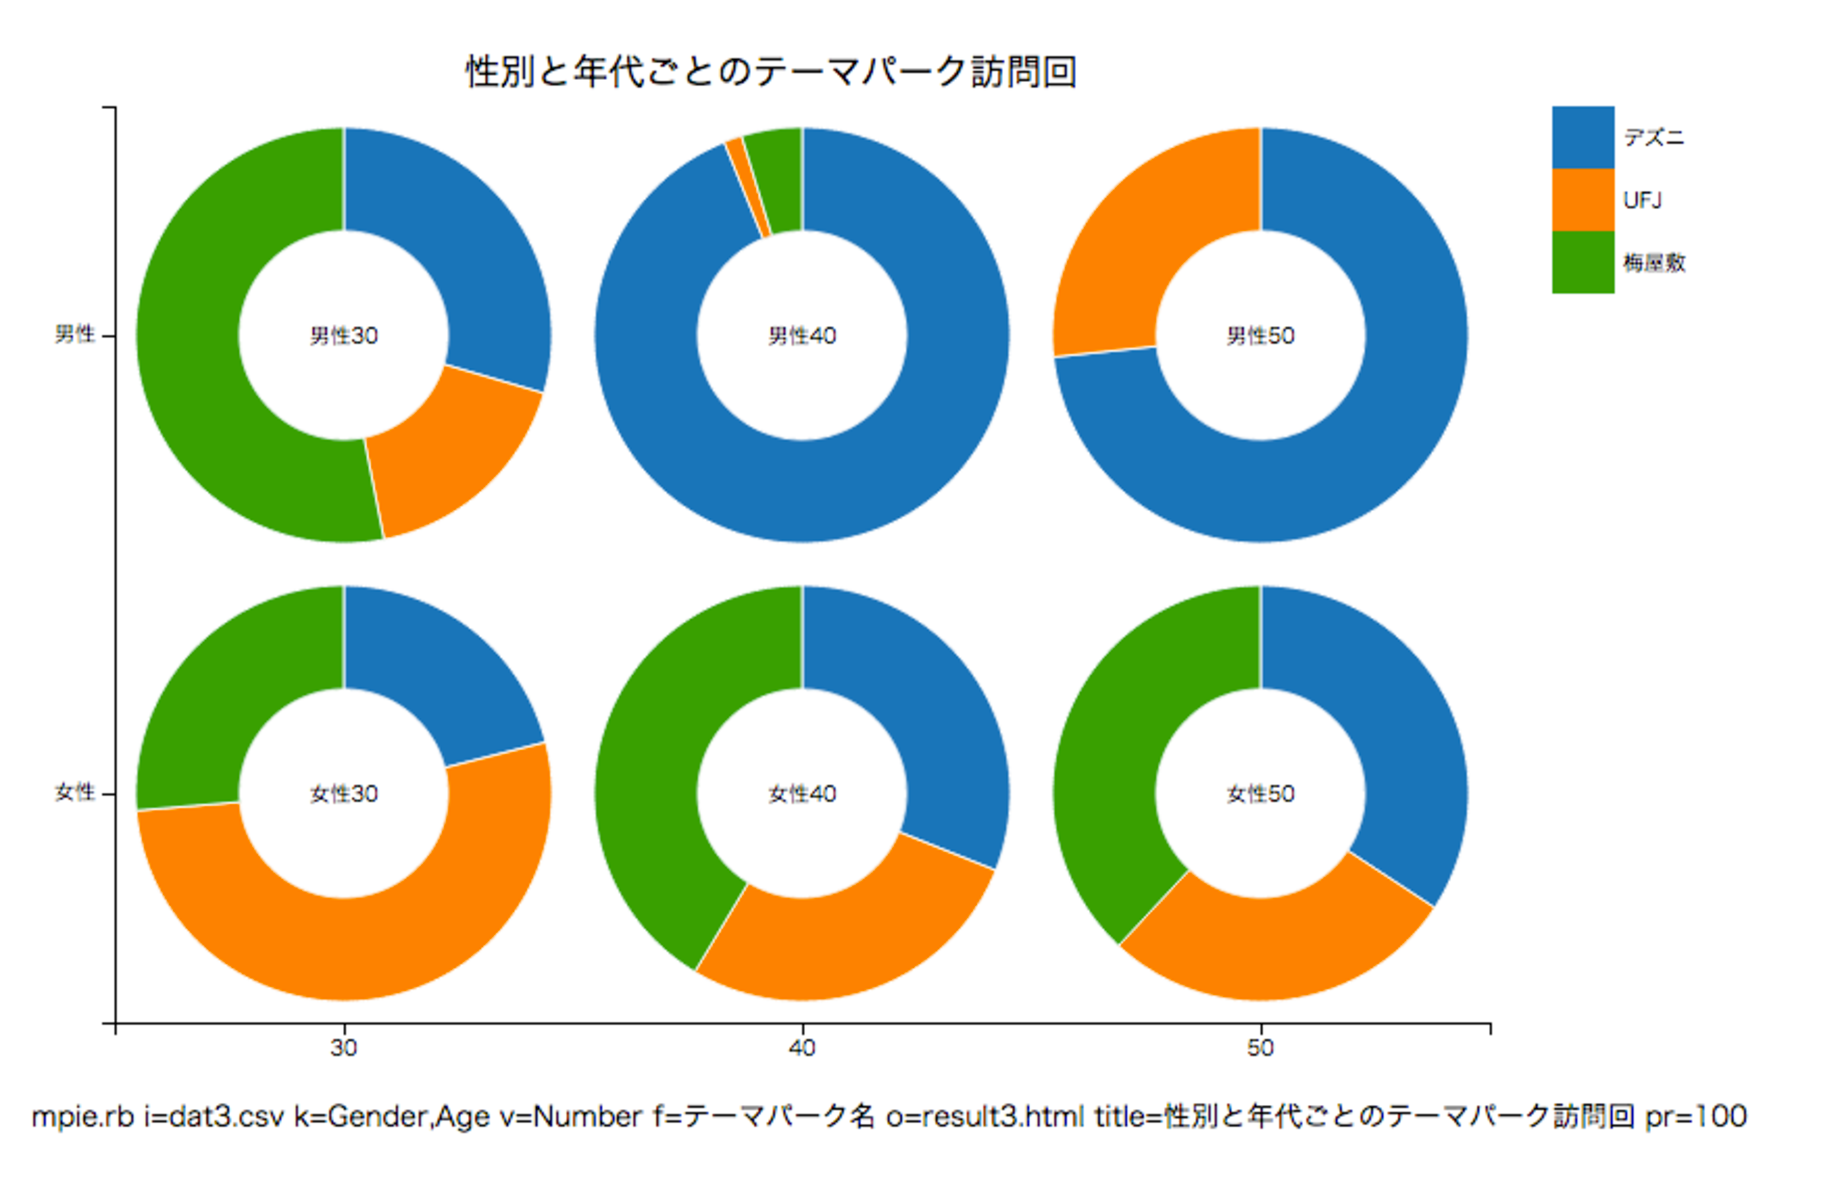
\includegraphics[scale=0.5]{figure/mpie3.eps}
}
\end{flushleft}


%\end{document}

